\section{Non Local Means (NLM)}
\frame{\sectionpage}
    
 \begin{frame}{Principle}

\begin{itemize}
    \item Iterative method
    \item Non Linear Filtering
    \item Using knowledge about neighbors
\end{itemize}

\end{frame}

\begin{frame}{Filter Expression}
\only<-2>{

    \uncover<+->{\begin{equation*}
    w(i, j, k, l) = - e^{\frac{\norm{I(i,j)-I(k,l)}^{2}_{2}}{2\sigma^{2}}}
    \end{equation*}}
    
    \uncover<+->{\begin{equation*}
    I_{D}(i,j) = \frac{\sum_{k,l} I(k,l) w(i,j,k,l)}{\sum_{k,l} w(i,j,k,l)}
    \end{equation*}}

}
\end{frame}

\begin{frame}{Algorithm}
\begin{algorithm}[H]
    \caption{Filtering Algorithm} % \label{euclid}
    \begin{algorithmic}[1]
        \Procedure{Denoising With Non Local Means Filter}{}\newline
        \textbf{Input:} $I$, $\sigma$, $(n_w, n_h)$ \\
        \textbf{Output:} $I_{D}$
        \For{\texttt{$pixel \in I$}}
            \State{$neighs = neighboors\_of(pixel, n_w, n_h)$}
            \State{$I_{D}[pixel] = non\_local\_mean(pixel, neighs, \sigma)$}
        \EndFor
        \EndProcedure
    \end{algorithmic}
    % \label{alg_1}
\end{algorithm}
\end{frame}

\begin{frame}{Data}
\centering
\begin{columns}
\column{.5\textwidth}
\centering
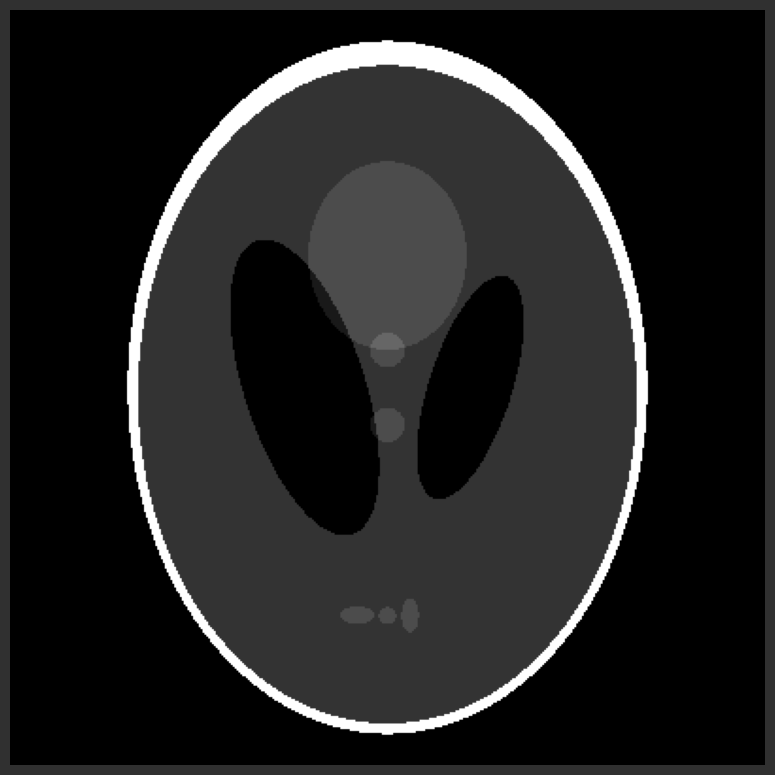
\includegraphics[scale=0.25]{images/results/original.png}
\column{.5\textwidth}
\centering
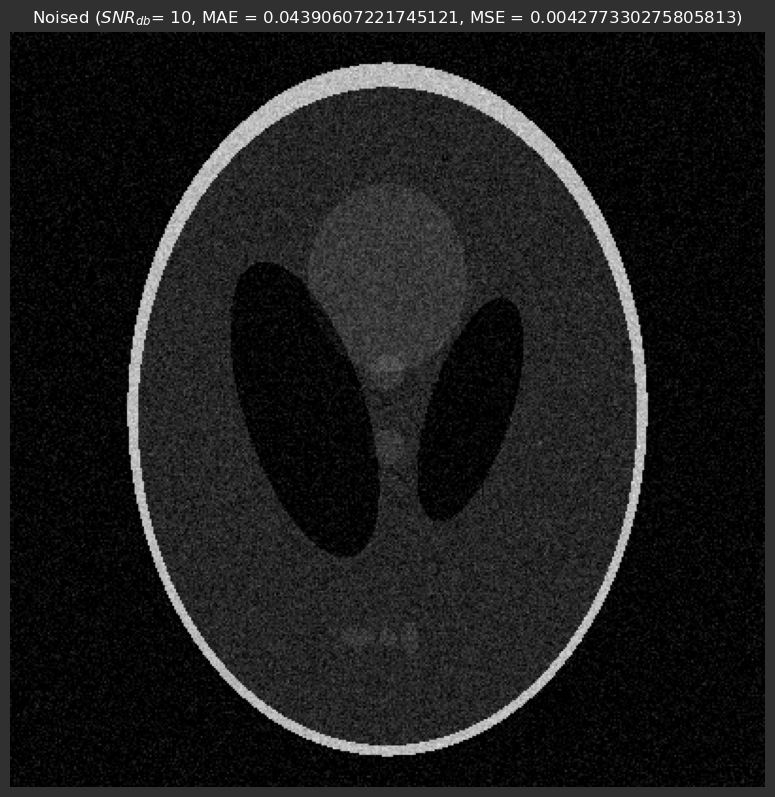
\includegraphics[scale=0.25]{images/results/noised.png}
\end{columns}
\end{frame}

\begin{frame}{Results (with $(n_w, n_h) = (5, 5)$)}
\centering
\begin{columns}
\column{.5\textwidth}
\centering
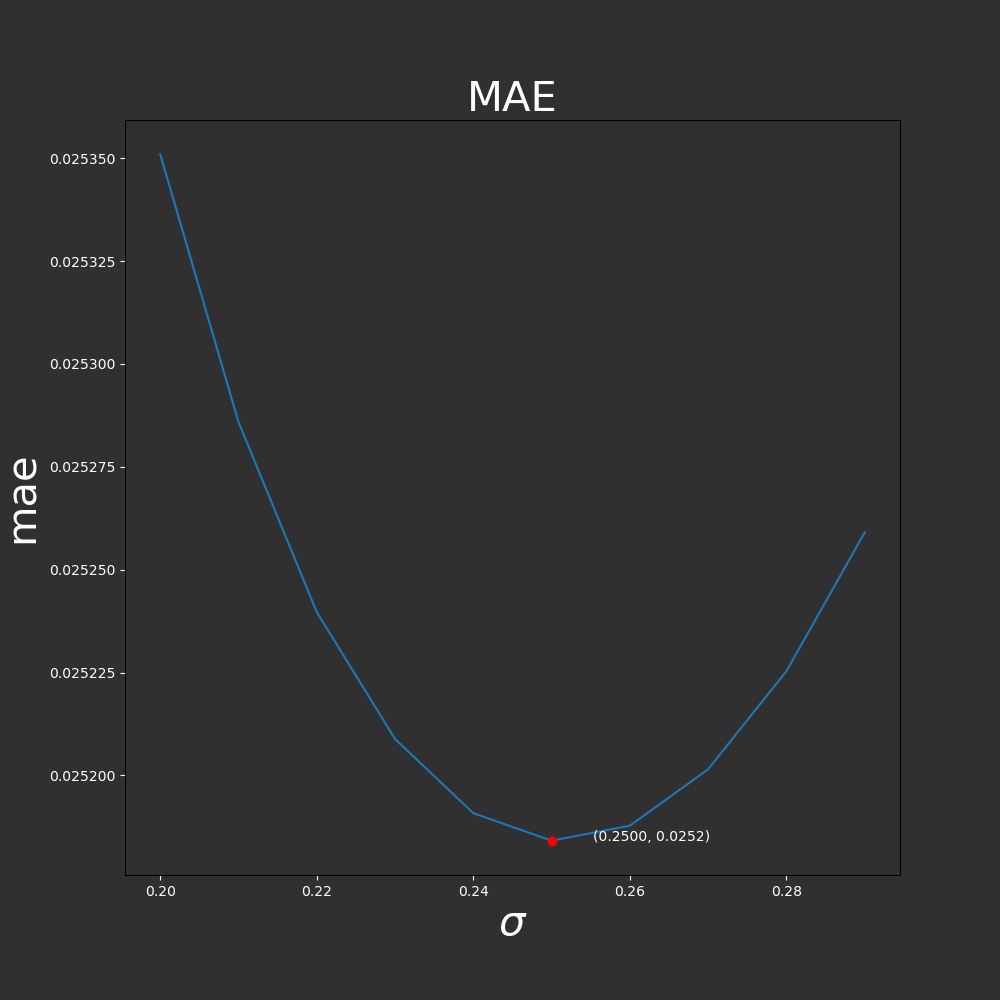
\includegraphics[scale=0.25]{images/results/nlm/plot_mae.png}
\column{.5\textwidth}
\centering
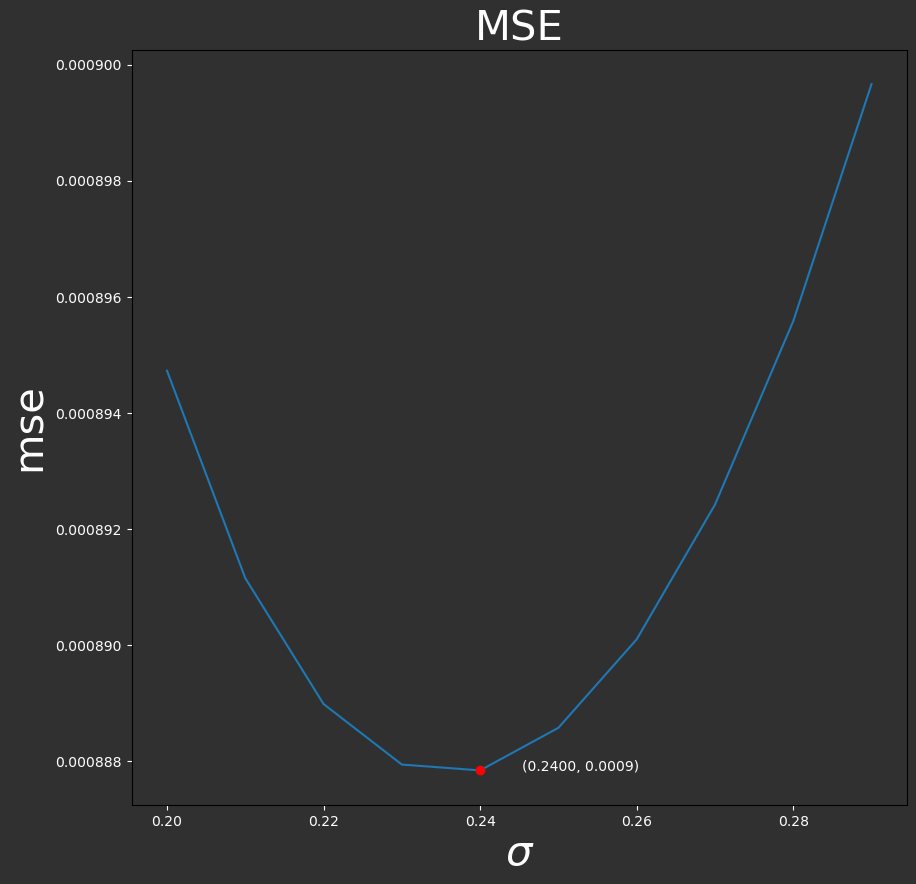
\includegraphics[scale=0.25]{images/results/nlm/plot_mse.png}
\end{columns}
\end{frame}

\begin{frame}{Results (with $(n_w, n_h) = (5, 5)$)}
\centering
\begin{columns}
\column{.5\textwidth}
\centering
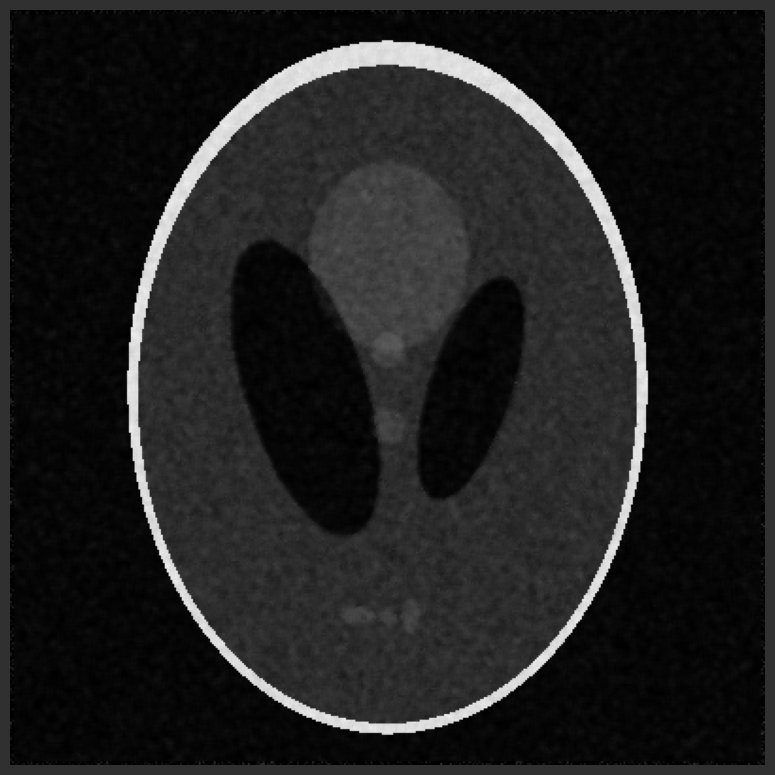
\includegraphics[scale=0.25]{images/results/nlm/image_mae.png}
\column{.5\textwidth}
\centering
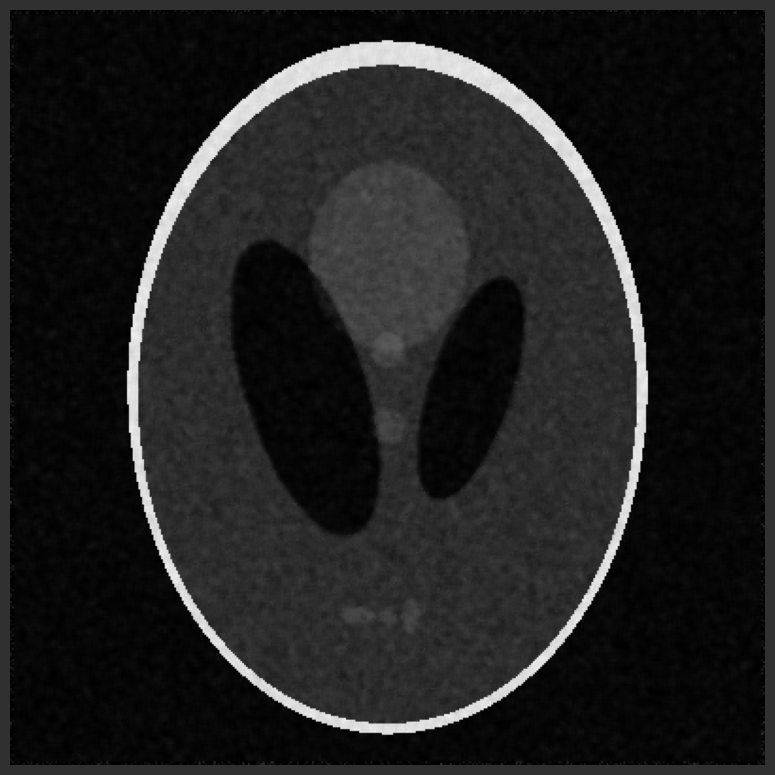
\includegraphics[scale=0.25]{images/results/nlm/image_mse.png}
\end{columns}
\end{frame}